\documentclass{article}
\usepackage[utf8]{inputenc}
\usepackage{graphicx}
\usepackage{amsmath}
\usepackage{hyperref}
\usepackage{float} % for positioning tables and figures

\title{Deep Learning for Sentiment Analysis and Machine Translation}
\author{Nguyen Viet Bac}
\date{June 2024}

\begin{document}

\maketitle

\begin{abstract}
This report explores the use of different deep learning models for two distinct NLP tasks: sentiment analysis and machine translation. For sentiment analysis, we compare Recurrent Neural Network (RNN), Transformer, and BERT models using the IMDB movie reviews dataset. For machine translation, we evaluate RNN-based Seq2Seq and Transformer models on the English-Vietnamese translation task. We assess the performance of each model and analyze their behavior in terms of accuracy, loss, BLEU score, and other relevant metrics. The results demonstrate the effectiveness of transformer-based models in both tasks.
\end{abstract}

\section{Introduction}
Natural Language Processing (NLP) encompasses a variety of tasks that enable machines to understand, interpret, and generate human language. This report focuses on two important NLP tasks: sentiment analysis and machine translation.

Sentiment analysis aims to determine the emotional tone behind a body of text, which can be useful for understanding customer opinions, feedback, and more. Machine translation involves translating text from one language to another, which is crucial for breaking language barriers in communication.

We employ deep learning models to tackle these tasks: Recurrent Neural Networks (RNNs), Transformers, and BERT for sentiment analysis, and Seq2Seq RNN and Transformer models for machine translation. We evaluate these models on the IMDB movie reviews dataset for sentiment analysis and the English-Vietnamese dataset for translation.

\section{Sentiment Analysis Methods}

Recurrent Neural Networks (RNNs) and Transformer models are widely used for sentiment analysis due to their ability to capture sequential dependencies and contextual information in text.

\subsection{Recurrent Neural Networks (RNNs)}
RNNs are effective for sentiment analysis because they can maintain a hidden state that captures information from previous words in the sequence, making them suitable for processing sequential data. Among RNN variants, we experimented with Long Short-Term Memory (LSTM) networks and Gated Recurrent Units (GRU), as well as bi-directional models.

\textbf{LSTM} networks are designed to combat the vanishing gradient problem by incorporating memory cells that can maintain information for long periods. This feature makes LSTMs particularly effective for capturing long-term dependencies in text sequences.

\textbf{GRU} networks are a simplified version of LSTM networks. They combine the forget and input gates into a single update gate, which simplifies the model and can lead to faster training times while still being capable of capturing long-range dependencies.

\textbf{Bi-directional RNNs} (including bi-directional LSTMs and GRUs) enhance the model's ability to capture context from both past and future words in the sequence. This is achieved by processing the input sequence in both forward and backward directions, which often results in better performance for tasks like sentiment analysis.

\subsection{Transformer Models}
Transformers have become the state-of-the-art approach for many NLP tasks due to their self-attention mechanism, which allows them to weigh the importance of different words in a sequence and capture long-range dependencies more efficiently than RNNs.

In our experiments, we utilized Transformers in two different capacities: standard implementation and fine-tuning a pre-trained model.

\textbf{Standard Transformer Implementation:} 
We implemented a standard Transformer model for sentiment analysis. This involved using the original Transformer architecture, which consists of an encoder-decoder structure with self-attention mechanisms to process the input text sequences.

\textbf{Fine-tuning with BERT:}
In addition to the standard implementation, we fine-tuned the pre-trained \textbf{BERT (Bidirectional Encoder Representations from Transformers)} model, specifically the 'bert-base-uncased' variant, for sentiment analysis. BERT is a transformer-based model pre-trained on a large corpus of text in an unsupervised manner, allowing it to develop a deep understanding of language.

\textbf{BERT-base-uncased} is a smaller version of BERT that is trained on lower-cased English text. Fine-tuning involves training the pre-trained BERT model on our specific sentiment analysis dataset, enabling it to adapt its learned representations to the nuances of our data. This approach leverages the power of transfer learning, where the model benefits from the extensive knowledge acquired during the pre-training phase.
\subsection{Summary of Methods}
\begin{itemize}
    \item \textbf{LSTM:} Captures long-term dependencies using memory cells.
    \item \textbf{GRU:} Simplified RNN variant that balances complexity and training efficiency.
    \item \textbf{Bi-directional RNNs:} Processes sequences in both directions for enhanced context.
    \item \textbf{Standard Transformer:} Implements the original Transformer architecture for sequence processing.
    \item \textbf{Fine-Tuned Transformer with BERT-base-uncased:} Utilizes self-attention for capturing long-range dependencies and benefits from transfer learning through fine-tuning.
\end{itemize}

These models were implemented and tested to evaluate their effectiveness in sentiment analysis, comparing their ability to understand and classify sentiments in textual data accurately.

\section{Sentiment Analysis Experiments}

\subsection{Dataset Details}
The IMDB Movie Reviews dataset is a binary sentiment analysis dataset containing 50,000 reviews from the Internet Movie Database (IMDB), each labeled as either positive or negative. The dataset has an equal number of positive and negative reviews. Only highly polarizing reviews are included: a negative review has a score of 4 or less out of 10, while a positive review has a score of 7 or more out of 10. No more than 30 reviews are included for any single movie.
Below are the first 5 samples from the training dataset:

\begin{figure}[H]
    \centering
    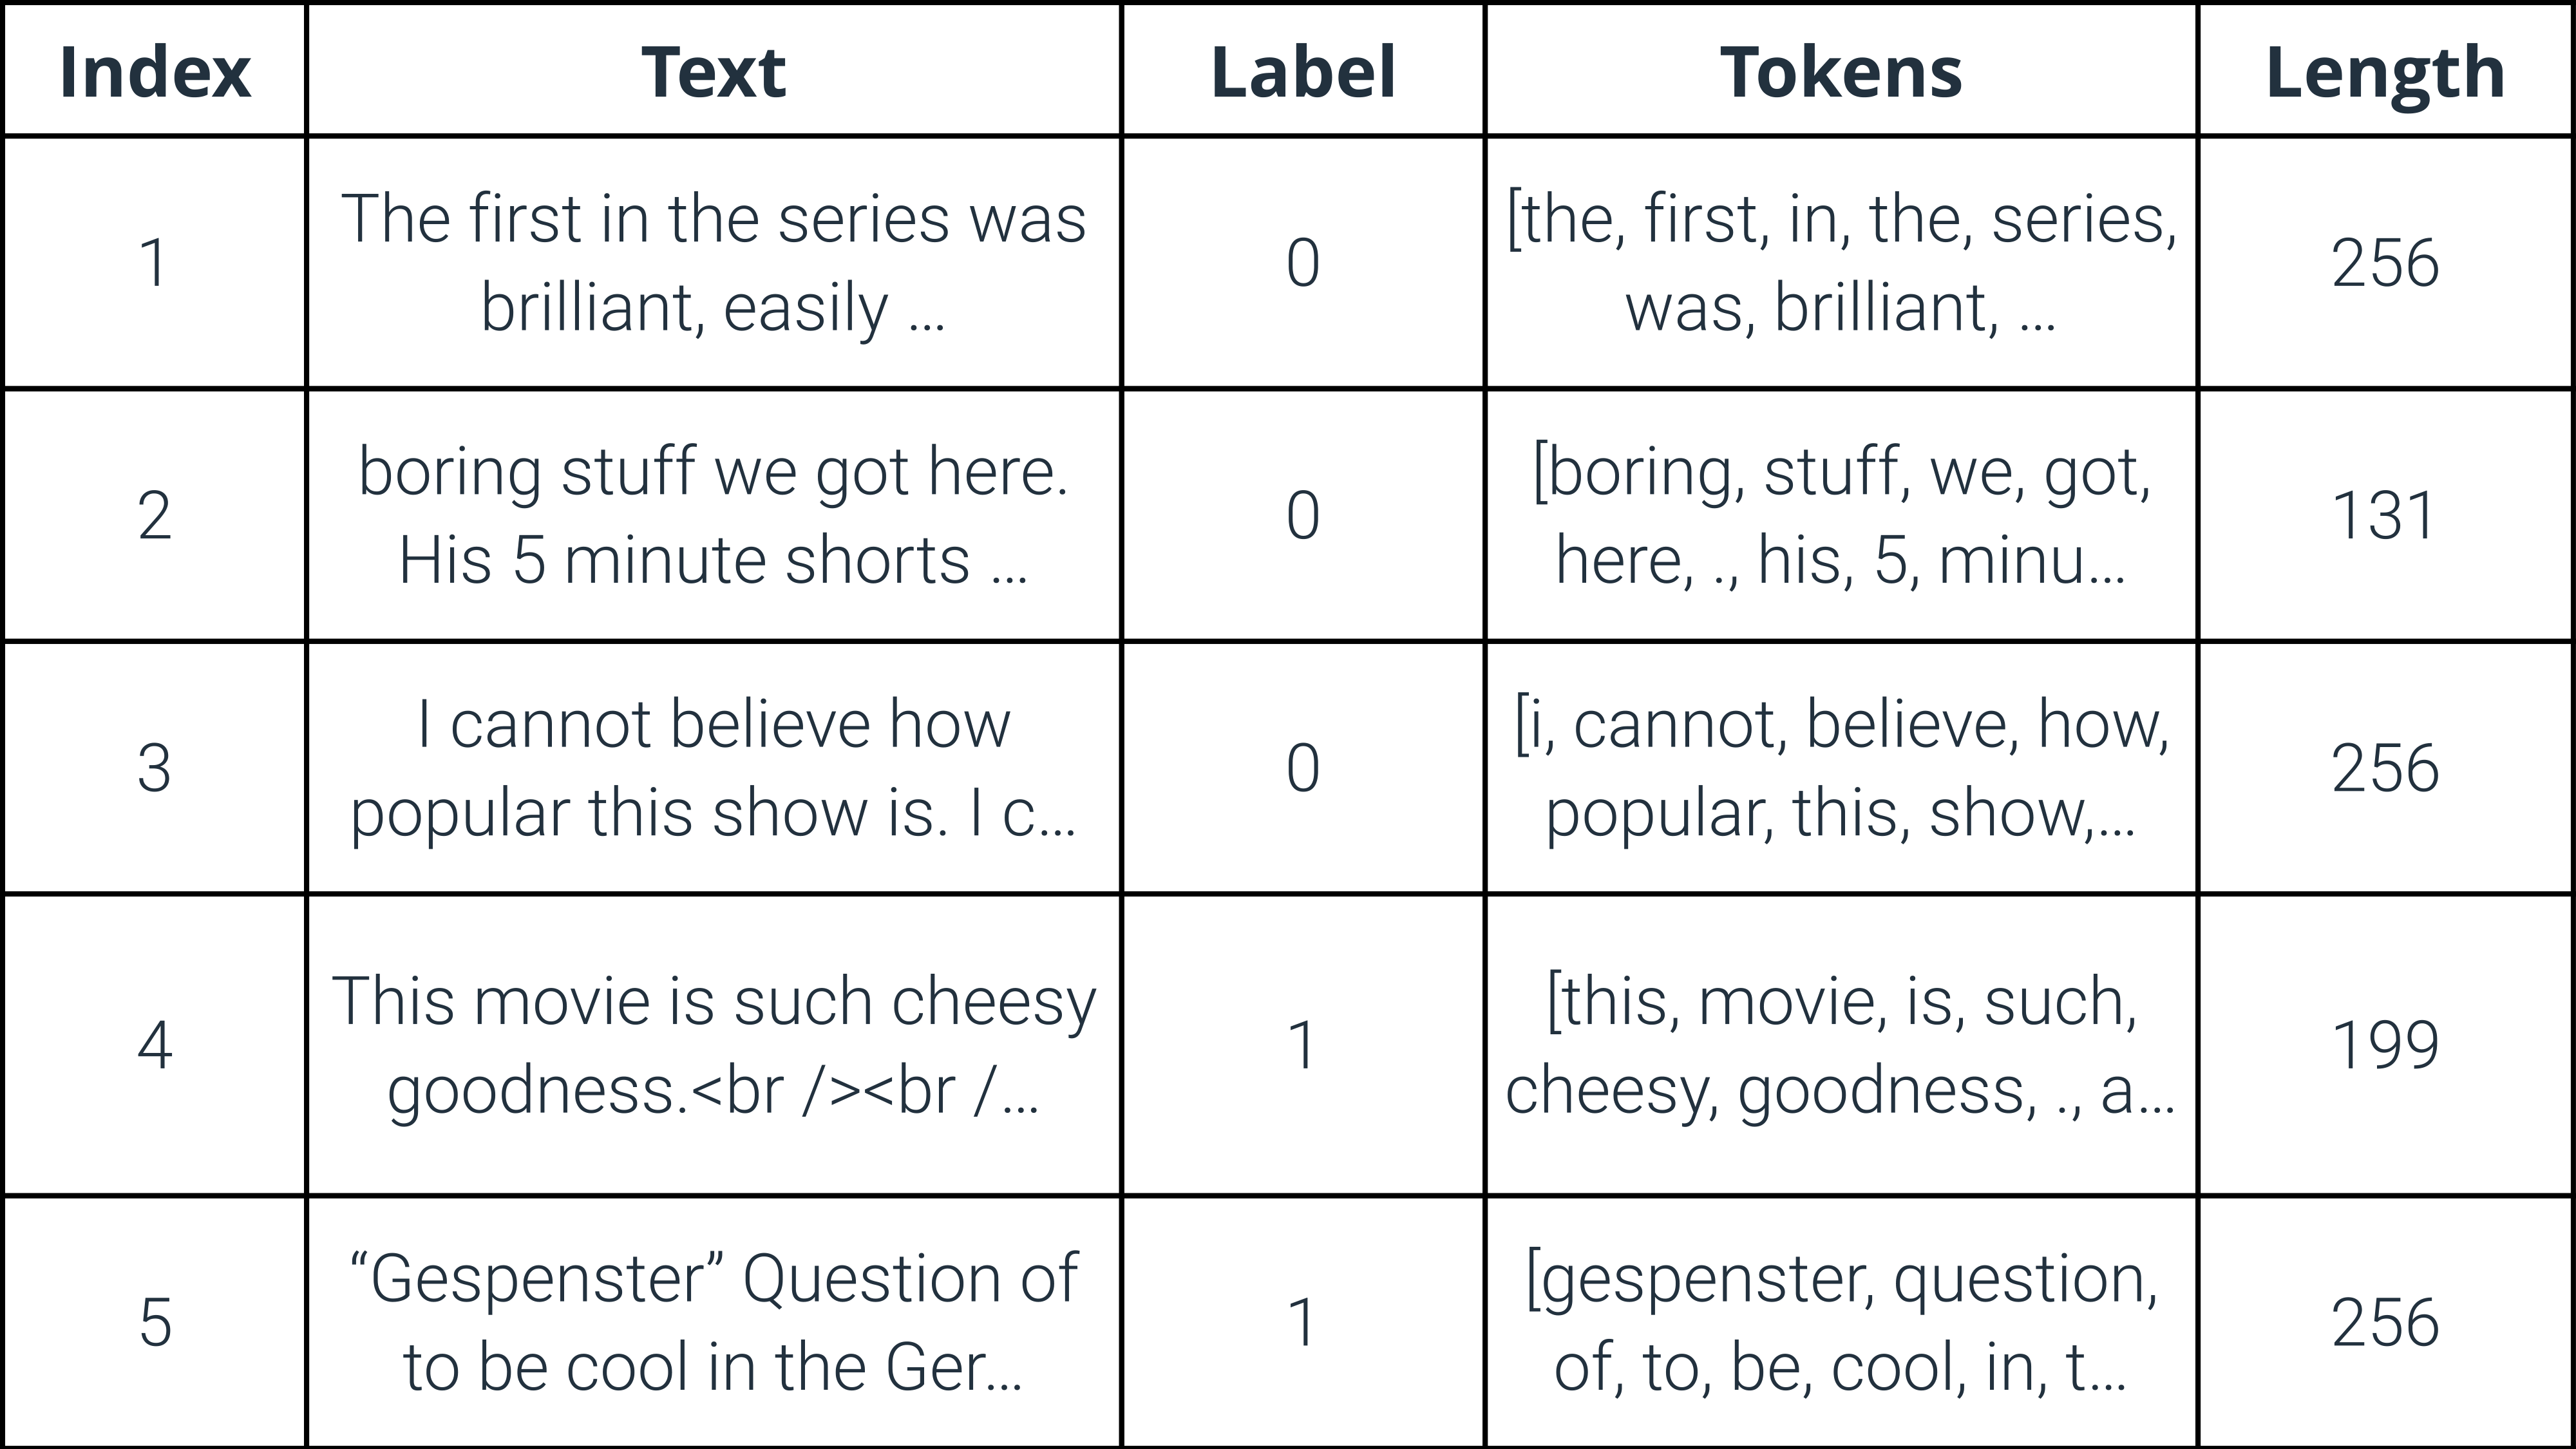
\includegraphics[width=\textwidth]{figs/head5imdb.png}
    \caption{First 5 Records of the Dataset}
    \label{fig:head5imdb}
\end{figure}
The provided samples illustrate the dataset's diversity in terms of review content and length. The tokenized texts exhibit varying lengths, with some reaching up to 256 tokens, highlighting the necessity for robust text processing techniques to manage variable input sizes. The sentiment labels are evenly distributed among these samples, reflecting the balanced nature of the dataset. The text snippets offer a glimpse into the range of sentiments, from highly critical to distinctly positive reviews. This balanced and varied dataset is ideally suited for training models in sentiment analysis, ensuring they can generalize well across different types of reviews.

\textbf{Dataset Shapes:}
\begin{itemize}
    \item \textbf{Training Set:} 17,500 reviews.
    \item \textbf{Validation Set:} 7,500 reviews.
    \item \textbf{Test Set:} 25,000 reviews. 
\end{itemize}

\subsection{Data Analysis}
To better understand the dataset, we visualize it using various plots.
\begin{figure}[H]
    \centering
    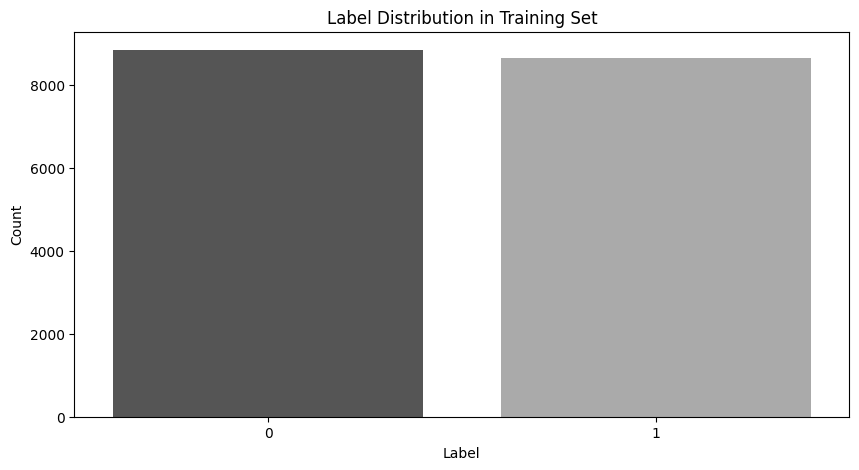
\includegraphics[width=\textwidth]{figs/laybelimdb.png}
    \caption{Label Distribution in Training Set}
    \label{fig:lengthimdb}
\end{figure}
Label Distribution Visualization
The provided bar chart depicts the label distribution within the training set of the IMDB Movie Reviews dataset. The x-axis represents the sentiment labels, with '0' indicating negative reviews and '1' indicating positive reviews. The y-axis represents the count of reviews for each label.

\textbf{Observations:}
The chart confirms an approximately equal number of positive and negative reviews in the training set. This balance is crucial for training effective sentiment analysis models, as it ensures that the model does not become biased toward a particular sentiment.
Both labels have counts close to 9,000, further indicating the balanced nature of the dataset. This equal representation helps in maintaining the model's performance across both classes during prediction.

\begin{figure}[H]
    \centering
    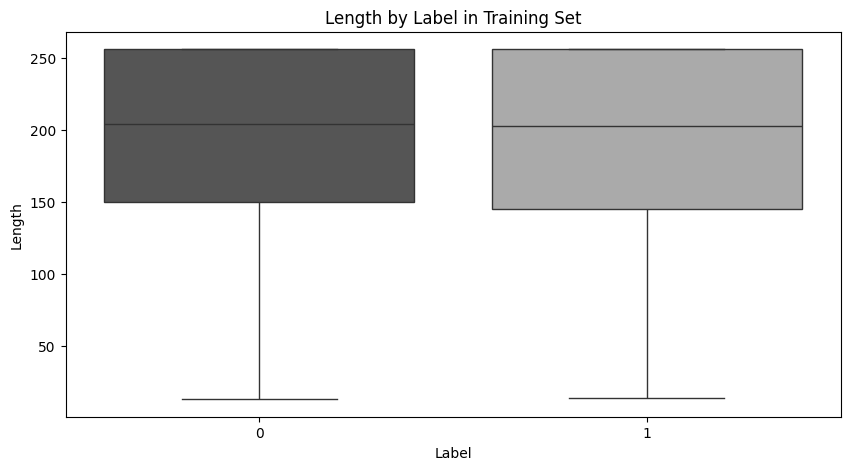
\includegraphics[width=\textwidth]{figs/lengthbylabelimdb.png}
    \caption{Length by Label in Training Set}
    \label{fig:lengthbylabelimdb}
\end{figure}

Both negative and positive reviews have a similar IQR, which suggests that the central 50\% of the review lengths are comparable in range for both sentiment labels.
The IQR for negative reviews extends from approximately 150 to 250 tokens.
The IQR for positive reviews extends from approximately 130 to 240 tokens.

The whiskers for both sentiment labels indicate the presence of reviews with lengths ranging from very short to quite long, with both having minimum lengths close to zero and maximum lengths around 256 tokens.
There are a few outliers present, particularly for the negative reviews, where some reviews are significantly shorter than the typical range.

The overall length distribution for both positive and negative reviews shows substantial overlap, indicating that review length alone may not be a distinguishing factor between the two sentiment labels.
Both distributions have a similar spread, suggesting that models will need to rely on the content of the reviews rather than their lengths to accurately predict sentiment.

\begin{figure}[H]
    \centering
    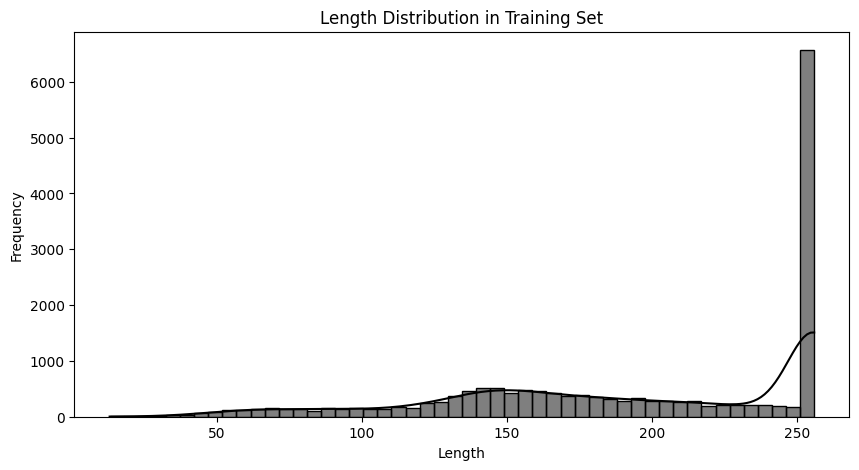
\includegraphics[width=\textwidth]{figs/lengthimdb.png}
    \caption{Length Distribution in Training Set}
    \label{fig:lengthimdb}
\end{figure}
The histogram illustrates that the review lengths are highly varied, with a substantial spike in frequency at the maximum review length of 250 words. This suggests that a significant portion of the reviews are either truncated or have exactly 250 words, possibly due to preprocessing or limitations in the dataset collection process.
The distribution also shows a smooth, albeit lower frequency, spread of review lengths below 100 words and above 150 words, before tapering off significantly past 200 words. The presence of a kernel density estimate (KDE) curve superimposed on the histogram further highlights these trends, smoothing out the variations to give a clearer view of the underlying distribution pattern.

\begin{figure}[H]
    \centering
    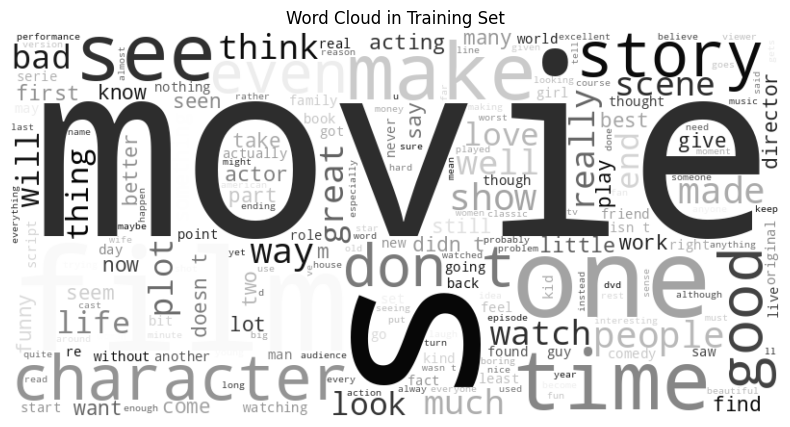
\includegraphics[width=\textwidth]{figs/wordcloudimdb.png}
    \caption{Word Cloud in Training Set}
    \label{fig:wordcloudimdb}
\end{figure}
The provided word cloud visualization represents the most frequently occurring words in the training set of the IMDB Movie Reviews dataset. The prominent presence and size of words such as "movie," "film," "story," "character," and "time" suggest these terms are central to the content of the reviews, reflecting common topics and themes discussed by reviewers.

\subsection{Model Settings}
The table below compares key settings for the models.

\begin{table}[H]
\centering
\begin{tabular}{|c|c|c|c|}
\hline
\textbf{Model} & \textbf{Batch Size} & \textbf{Epochs} & \textbf{Learning Rate} \\
\hline
RNN & 128 & 10 & 0.001 \\
LSTM & 128 & 10 & 0.001 \\
GRU & 128 & 10 & 0.001 \\
Bidirectional LSTM & 128 & 5 & 0.001 \\
Transformer & 128 & 5 & 0.001 \\
Fine-Tuned Transformer & 8 & 3 & 0.00001 \\
\hline
\end{tabular}
\caption{Comparison of Model Settings}
\label{table:model-settings}
\end{table}

\begin{table}[H]
\centering
\begin{tabular}{|c|c|c|}
\hline
\textbf{Model} & \textbf{Loss Function} & \textbf{Optimizer} \\
\hline
RNN & Binary Cross-Entropy & Adam \\
LSTM & Binary Cross-Entropy & Adam \\
GRU & Binary Cross-Entropy & Adam \\
Bidirectional LSTM & Binary Cross-Entropy & Adam \\
Transformer & Binary Cross-Entropy & Adam \\
Fine-Tuned Transformer & Cross-Entropy Loss & Adam \\
\hline
\end{tabular}
\caption{Comparison of Loss Functions and Optimizers}
\label{table:loss-optimizer}
\end{table}
The epoch count for the fine-tuned Transformer was intentionally kept low at 3 epochs due to extended training durations associated with Transformer architectures, especially when fine-tuning pre-trained models. This decision aimed to achieve a reasonable trade-off between achieving convergence and minimizing computational overhead. By focusing on a reduced number of epochs with meticulous tuning of hyperparameters like learning rates, we aimed to ensure that the model could effectively capture sentiment nuances without excessively prolonging training times.

Moreover, the batch size of 8 was chosen for the fine-tuned Transformer to facilitate fine-grained adjustments during training, enhancing its ability to generalize well to sentiment analysis tasks. This setup not only streamlined the training process but also contributed to achieving competitive performance metrics such as accuracy and F1 score on sentiment classification tasks.

\subsubsection{RNN}
Recurrent Neural Networks (RNNs) process sequential data by maintaining a hidden state that captures information about previous elements in the sequence.

\begin{itemize}
    \item \textbf{Embedding Layer:} Converts input words to dense vectors.
    \item \textbf{SimpleRNN Layer:} One layer with 32 hidden units.
    \item \textbf{Fully Connected Layer:} Maps the RNN output to the output classes.
\end{itemize}

\subsubsection{LSTM}
Long Short-Term Memory (LSTM) networks are capable of learning long-term dependencies.

\begin{itemize}
    \item \textbf{Embedding Layer:} Converts input words to dense vectors.
    \item \textbf{LSTM Layers:} One layer with 300 hidden units.
    \item \textbf{Dropout:} A dropout rate of 0.5 to prevent overfitting.
    \item \textbf{Fully Connected Layer:} Maps the LSTM output to the output classes.
\end{itemize}

\subsubsection{GRU}
Gated Recurrent Unit (GRU) networks simplify the LSTM architecture while maintaining performance.

\begin{itemize}
    \item \textbf{Embedding Layer:} Converts input words to dense vectors.
    \item \textbf{GRU Layer:} One layer with 16 hidden units.
    \item \textbf{Fully Connected Layer:} Maps the GRU output to the output classes.
\end{itemize}

\subsubsection{Bidirectional LSTM}
Bidirectional LSTMs process the data in both forward and backward directions.

\begin{itemize}
    \item \textbf{Embedding Layer:} Converts input words to dense vectors.
    \item \textbf{Bidirectional LSTM Layer:} One layer with 64 hidden units.
    \item \textbf{Fully Connected Layer:} Maps the Bidirectional LSTM output to the output classes.
\end{itemize}

\subsubsection{Transformer}
Transformers use self-attention mechanisms to weigh the importance of different words in a sequence, capturing long-range dependencies efficiently.

\begin{itemize}
    \item \textbf{Model:} Custom transformer architecture with 8 attention heads and 256 feed-forward units.
    \item \textbf{Self-Attention:} Multi-head self-attention with 8 attention heads.
    \item \textbf{Dropout Rate:} 0.1.
    \item \textbf{Output Layer:} Dense layer with 20 units and ReLU activation, followed by a dropout layer and a final dense layer with sigmoid activation.
\end{itemize}

\subsubsection{Fine-Tuned Transformer}
Fine-tuning a pre-trained transformer model (BERT) for classification tasks.

\begin{itemize}
    \item \textbf{Model:} \texttt{bert-base-uncased} from Hugging Face.
    \item \textbf{Tokenizer:} Tokenizer from \texttt{bert-base-uncased}.
    \item \textbf{Architecture:} Transformer with a linear layer on top for classification.
\end{itemize}

\subsection{Results}
The comparative analysis of model performance in Table \ref{table:model-results} underscores the significant variations in test accuracy among the different architectures applied in this study. The dataset was evaluated using several neural network models, including Recurrent Neural Networks (RNN), Long Short-Term Memory networks (LSTM), Gated Recurrent Units (GRU), Bidirectional LSTMs, and Transformers. These models were selected for their distinct capabilities in handling sequential data, a common characteristic in many machine learning tasks.

\begin{table}[H]
\centering
\begin{tabular}{|c|c|}
\hline
\textbf{Model} & \textbf{Test Accuracy (\%)} \\
\hline
RNN & 82.82 \\
LSTM & 85.84 \\
GRU & 84.01 \\
Bidirectional LSTM & 86.96 \\
Transformer & 85.55 \\
Fine-Tuned Transformer & 92.80 \\
\hline
\end{tabular}
\caption{Comparison of Model Performance}
\label{table:model-results}
\end{table}
In this study, the Fine-Tuned Transformer model significantly outperforms all other models, achieving a test accuracy of 92.80\%. This highlights the efficacy of transfer learning and the potential of pre-trained models in achieving superior performance in specific tasks. The Bidirectional LSTM also demonstrates robust performance with an accuracy of 86.96\%, reflecting the advantage of processing information in both forward and backward directions. Traditional LSTMs and GRUs show competitive accuracies of 85.84\% and 84.01\% respectively, indicating their effectiveness in handling sequential data. The baseline RNN model, while the least accurate, still achieves a respectable 82.82\%, showcasing the fundamental capability of recurrent architectures.

\subsection{Evaluation of Fine-Tuned Transformer Model}
To evaluate the performance of the Fine-Tuned Transformer Model, we conducted a series of sentiment tests. The table below presents a comparison between the predicted sentiment and the label for a set of sample inputs.
\begin{figure}[H]
    \centering
    \includegraphics[width=\textwidth]{figs/transformer.png}
    \caption{Sentiment Analysis Results from Fine-Tuned Transformer Model}
    \label{fig:transformer-evaluation}
\end{figure}
Illustrate the effectiveness of the Fine-Tuned Transformer Model in sentiment analysis. The model demonstrates a high degree of accuracy in predicting the sentiment of review sentences, as evidenced by the close alignment between predicted sentiments and the actual labels. The probability scores accompanying the predictions further highlight the model's confidence in its classifications.

The Fine-Tuned Transformer Model's robust performance can be attributed to its advanced architecture, which leverages pre-trained knowledge and fine-tuning techniques to enhance its understanding of nuanced language patterns. This capability allows the model to effectively interpret and classify complex sentiments, making it a powerful tool for sentiment analysis tasks.

Despite the overall strong performance, there were instances where the model's predictions did not align with the actual labels. The table below presents examples of such cases.
\begin{figure}[H]
    \centering
    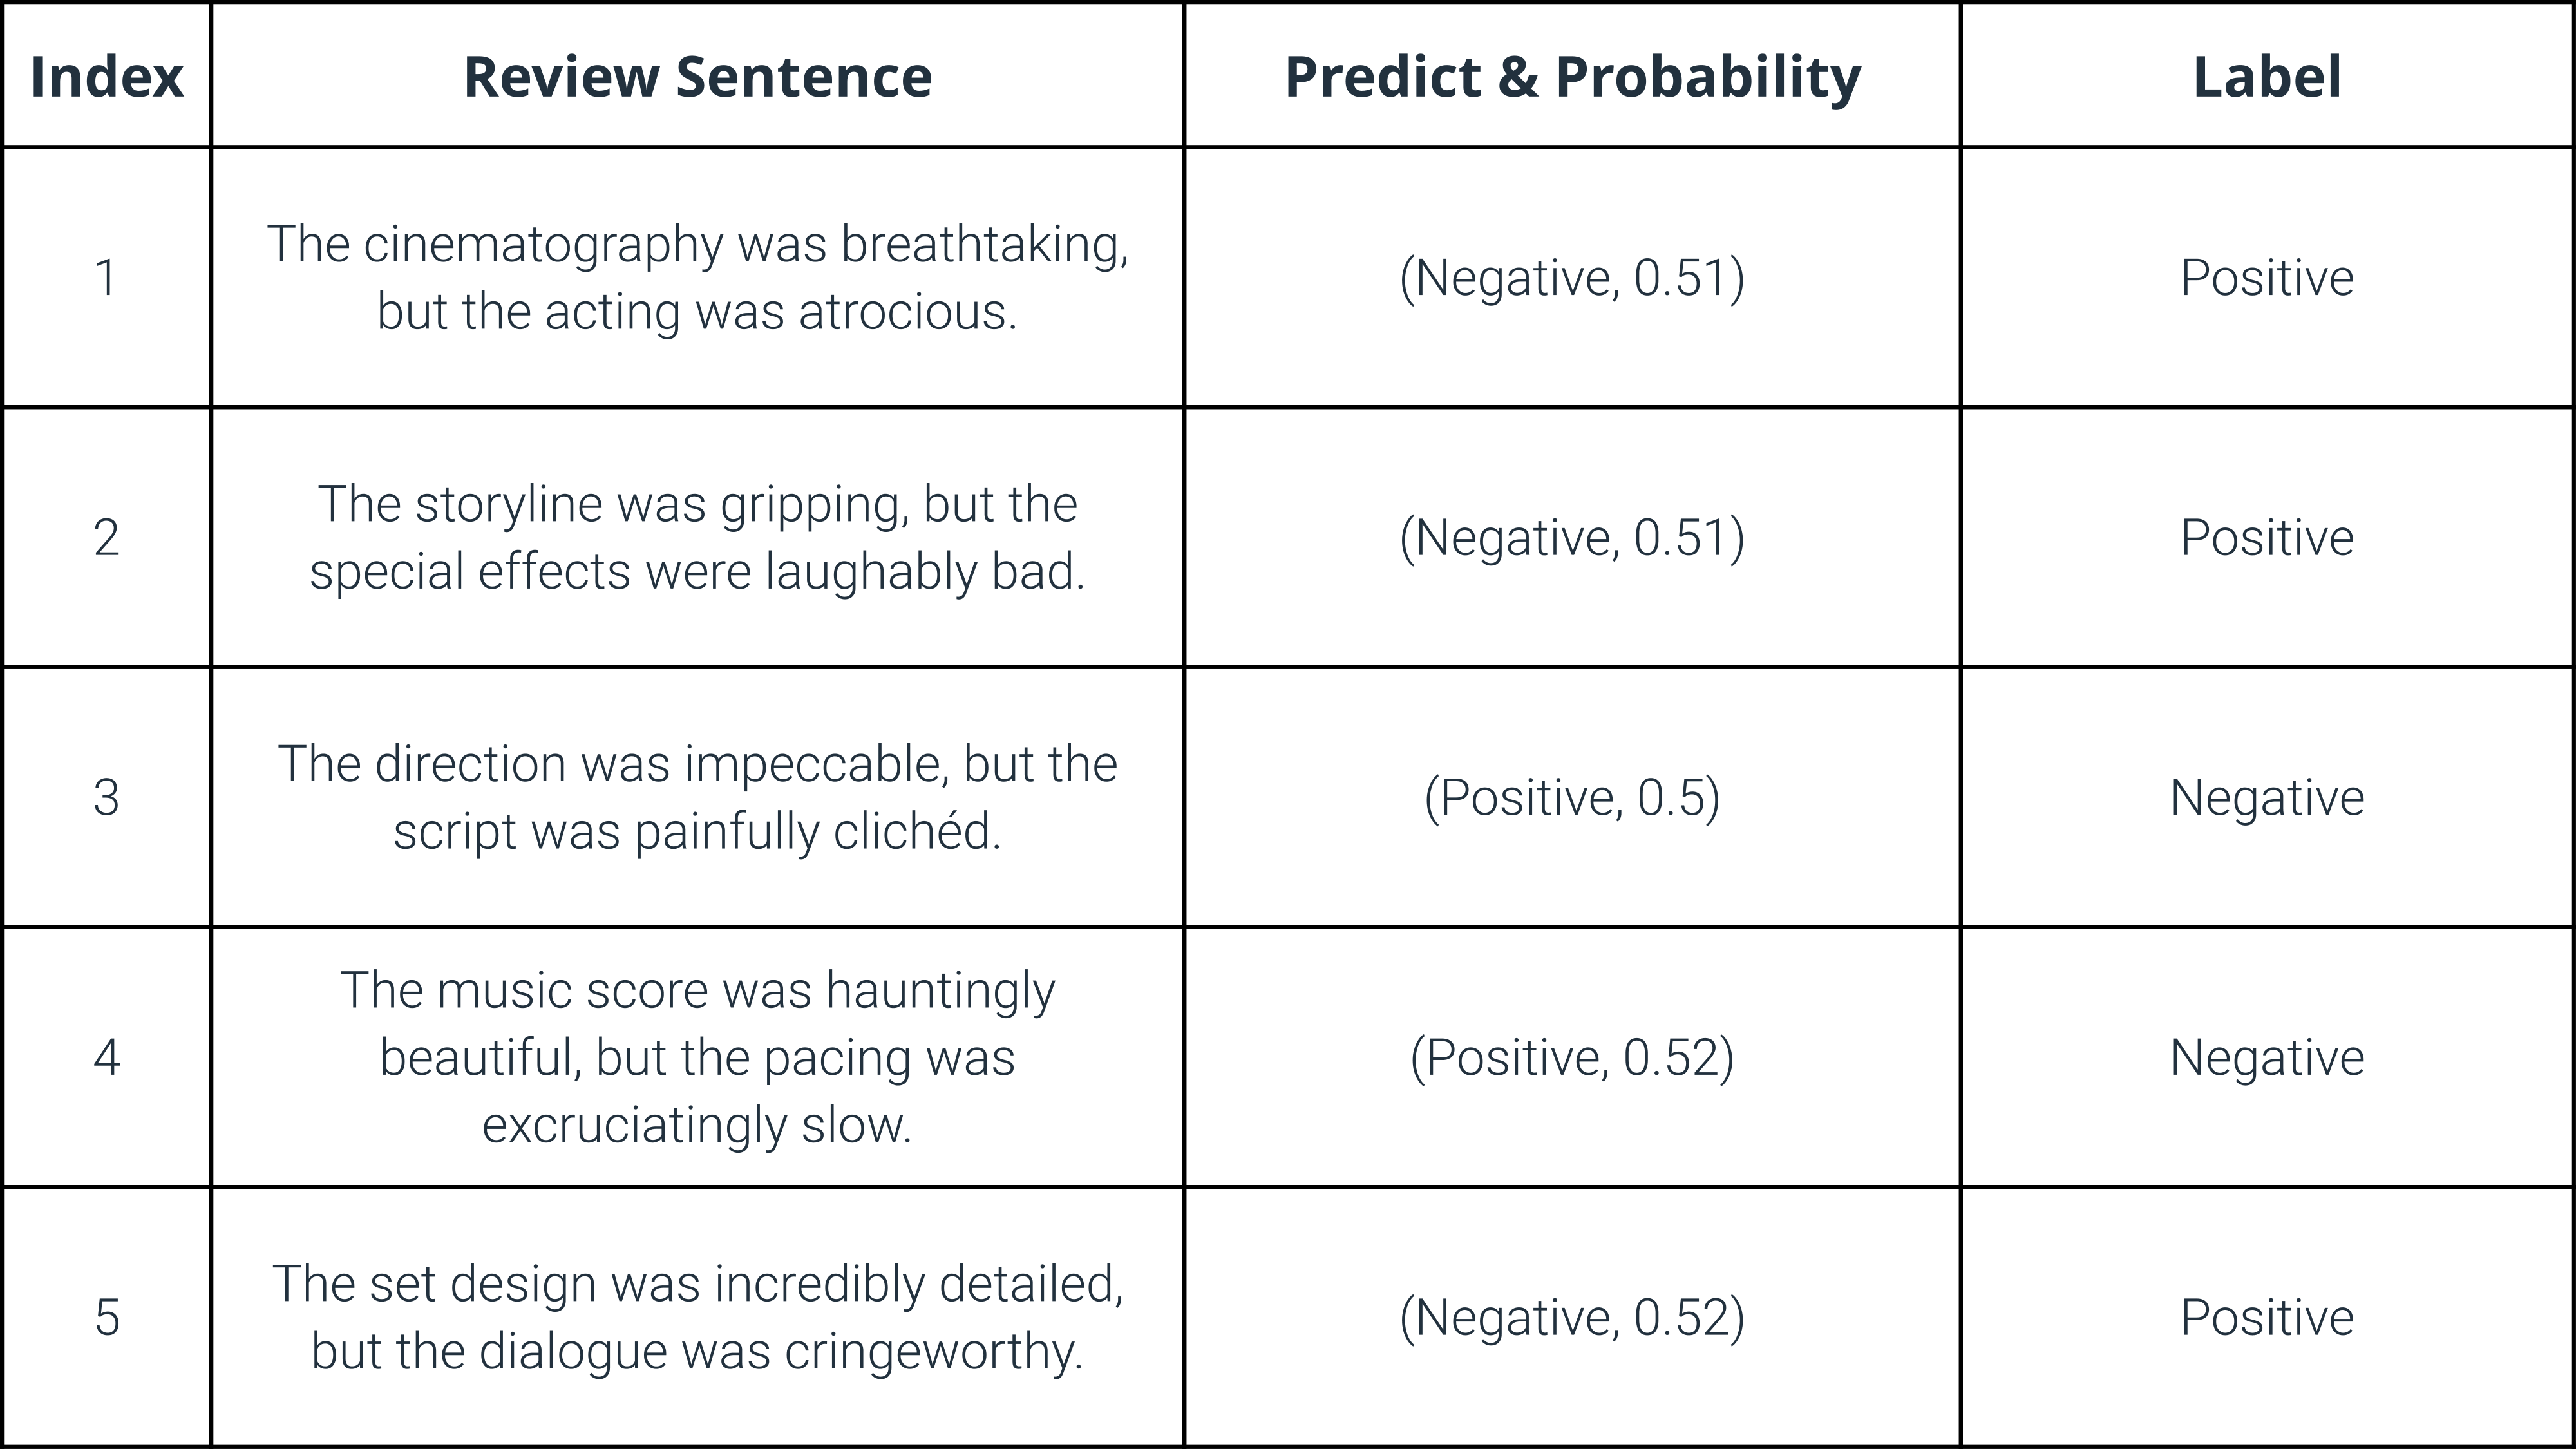
\includegraphics[width=\textwidth]{figs/wrong.png}
    \caption{Examples of Incorrect Sentiment Predictions by the Fine-Tuned Transformer Model}
    \label{fig:wrong-predictions}
\end{figure}

In analyzing the sentences where the model's predictions were incorrect, several factors can be identified as potential reasons for these errors:
\begin{itemize}
    \item \textbf{Contradictory Sentiment Cues}: Many of the incorrectly predicted sentences contain contradictory sentiment cues. For example, a sentence may start with a positive attribute but end with a strong negative critique. This duality can confuse the model, which might focus on the more dominant sentiment component in its training set.
    \item \textbf{Subtle Negations and Sarcasm}: Some sentences include subtle negations or sarcastic undertones that are difficult for the model to detect. For instance, phrases like “painfully clichéd” or “laughably bad” may appear positive at a superficial level but are actually negative in context.
    \item \textbf{Contextual Complexity}: The presence of complex contextual relationships within a sentence, where the sentiment depends heavily on the specific combination of words, can also lead to misclassification. The model might miss these nuanced connections, leading to incorrect predictions.
    \item \textbf{Probability Threshold Margins}: The predictions in some cases were very close to the decision boundary (around 50\% probability), indicating a lack of strong confidence in either direction. These borderline cases highlight the challenge in interpreting sentiments that are not distinctly positive or negative.
\end{itemize}

Understanding these nuances can provide valuable insights into areas where the model could be further refined, potentially leading to even more accurate sentiment analysis in future applications.


\section{Machine Translation Methods}
RNN-based Seq2Seq and Transformer models are used for machine translation due to their ability to handle sequential data and capture dependencies between words in a sentence.

\textbf{RNN-based Seq2Seq} models are effective for translation tasks as they can process input sequences and generate corresponding output sequences, maintaining contextual information throughout the sequence with their hidden states.

\textbf{Transformers} provide an advantage in translation tasks due to their self-attention mechanism, which allows them to process entire sequences simultaneously and capture dependencies between all words in a sentence, resulting in more accurate translations.

In addition to these methods, we also utilize the pre-trained model \textbf{MarianMTModel} for our project.

The \textbf{MarianMTModel} is particularly well-suited for machine translation tasks due to several key reasons:

Pre-training on Diverse Data: MarianMTModel is pre-trained on a vast amount of multilingual data, enabling it to handle a wide range of languages and translation pairs effectively. This extensive pre-training helps the model to generalize well and produce high-quality translations.

Efficient Architecture: The MarianMTModel leverages the Transformer architecture, which benefits from parallel processing and the self-attention mechanism, making it highly efficient and capable of capturing long-range dependencies in sentences. This results in translations that are both fast and accurate.

Fine-Tuning Capabilities: MarianMTModel can be fine-tuned on specific datasets, allowing it to adapt to particular translation tasks and domains. This customization ensures that the translations meet the specific requirements of the project, improving both relevance and accuracy.

State-of-the-Art Performance: As a pre-trained model from the Marian NMT framework, MarianMTModel has demonstrated state-of-the-art performance in various translation benchmarks. Its robustness and reliability make it a preferred choice for machine translation applications.

By incorporating the MarianMTModel, our project leverages these advantages to achieve superior translation quality, enhancing the overall effectiveness of our machine translation system.

\section{Machine Translation Experiments}

\subsection{Dataset Details}
The dataset named "Machine Translation Paired English-Vietnamese Sentences" is a valuable resource for projects involving machine translation between English and Vietnamese. It contains a substantial volume of data, categorized within the 1 million to 10 million size range, making it suitable for training and evaluating robust translation models.

This dataset is sourced from various reputable origins, including Open Subtitles, Tatoeba, OPUS TED Talks, QED Amara, and OPUS Wikipedia, ensuring a diverse and comprehensive collection of sentence pairs. The data was curated and annotated through a combination of found annotations and language creation methods, emphasizing its authenticity and reliability.

It is designed specifically for tasks related to conditional text generation, with a primary focus on machine translation. The multilingual nature of the dataset supports translation between English (en) and Vietnamese (vi), catering to the needs of developers and researchers working on bilingual translation systems.

Licensed under the MIT license, this dataset is open for public use, allowing for wide dissemination and application in various translation projects. The name "Machine Translation Paired English-Vietnamese Sentences" aptly reflects its content and purpose, offering an extensive repository of sentence pairs for enhancing translation technologies.
Below are the first 5 samples from the training dataset:

\begin{figure}[H]
    \centering
    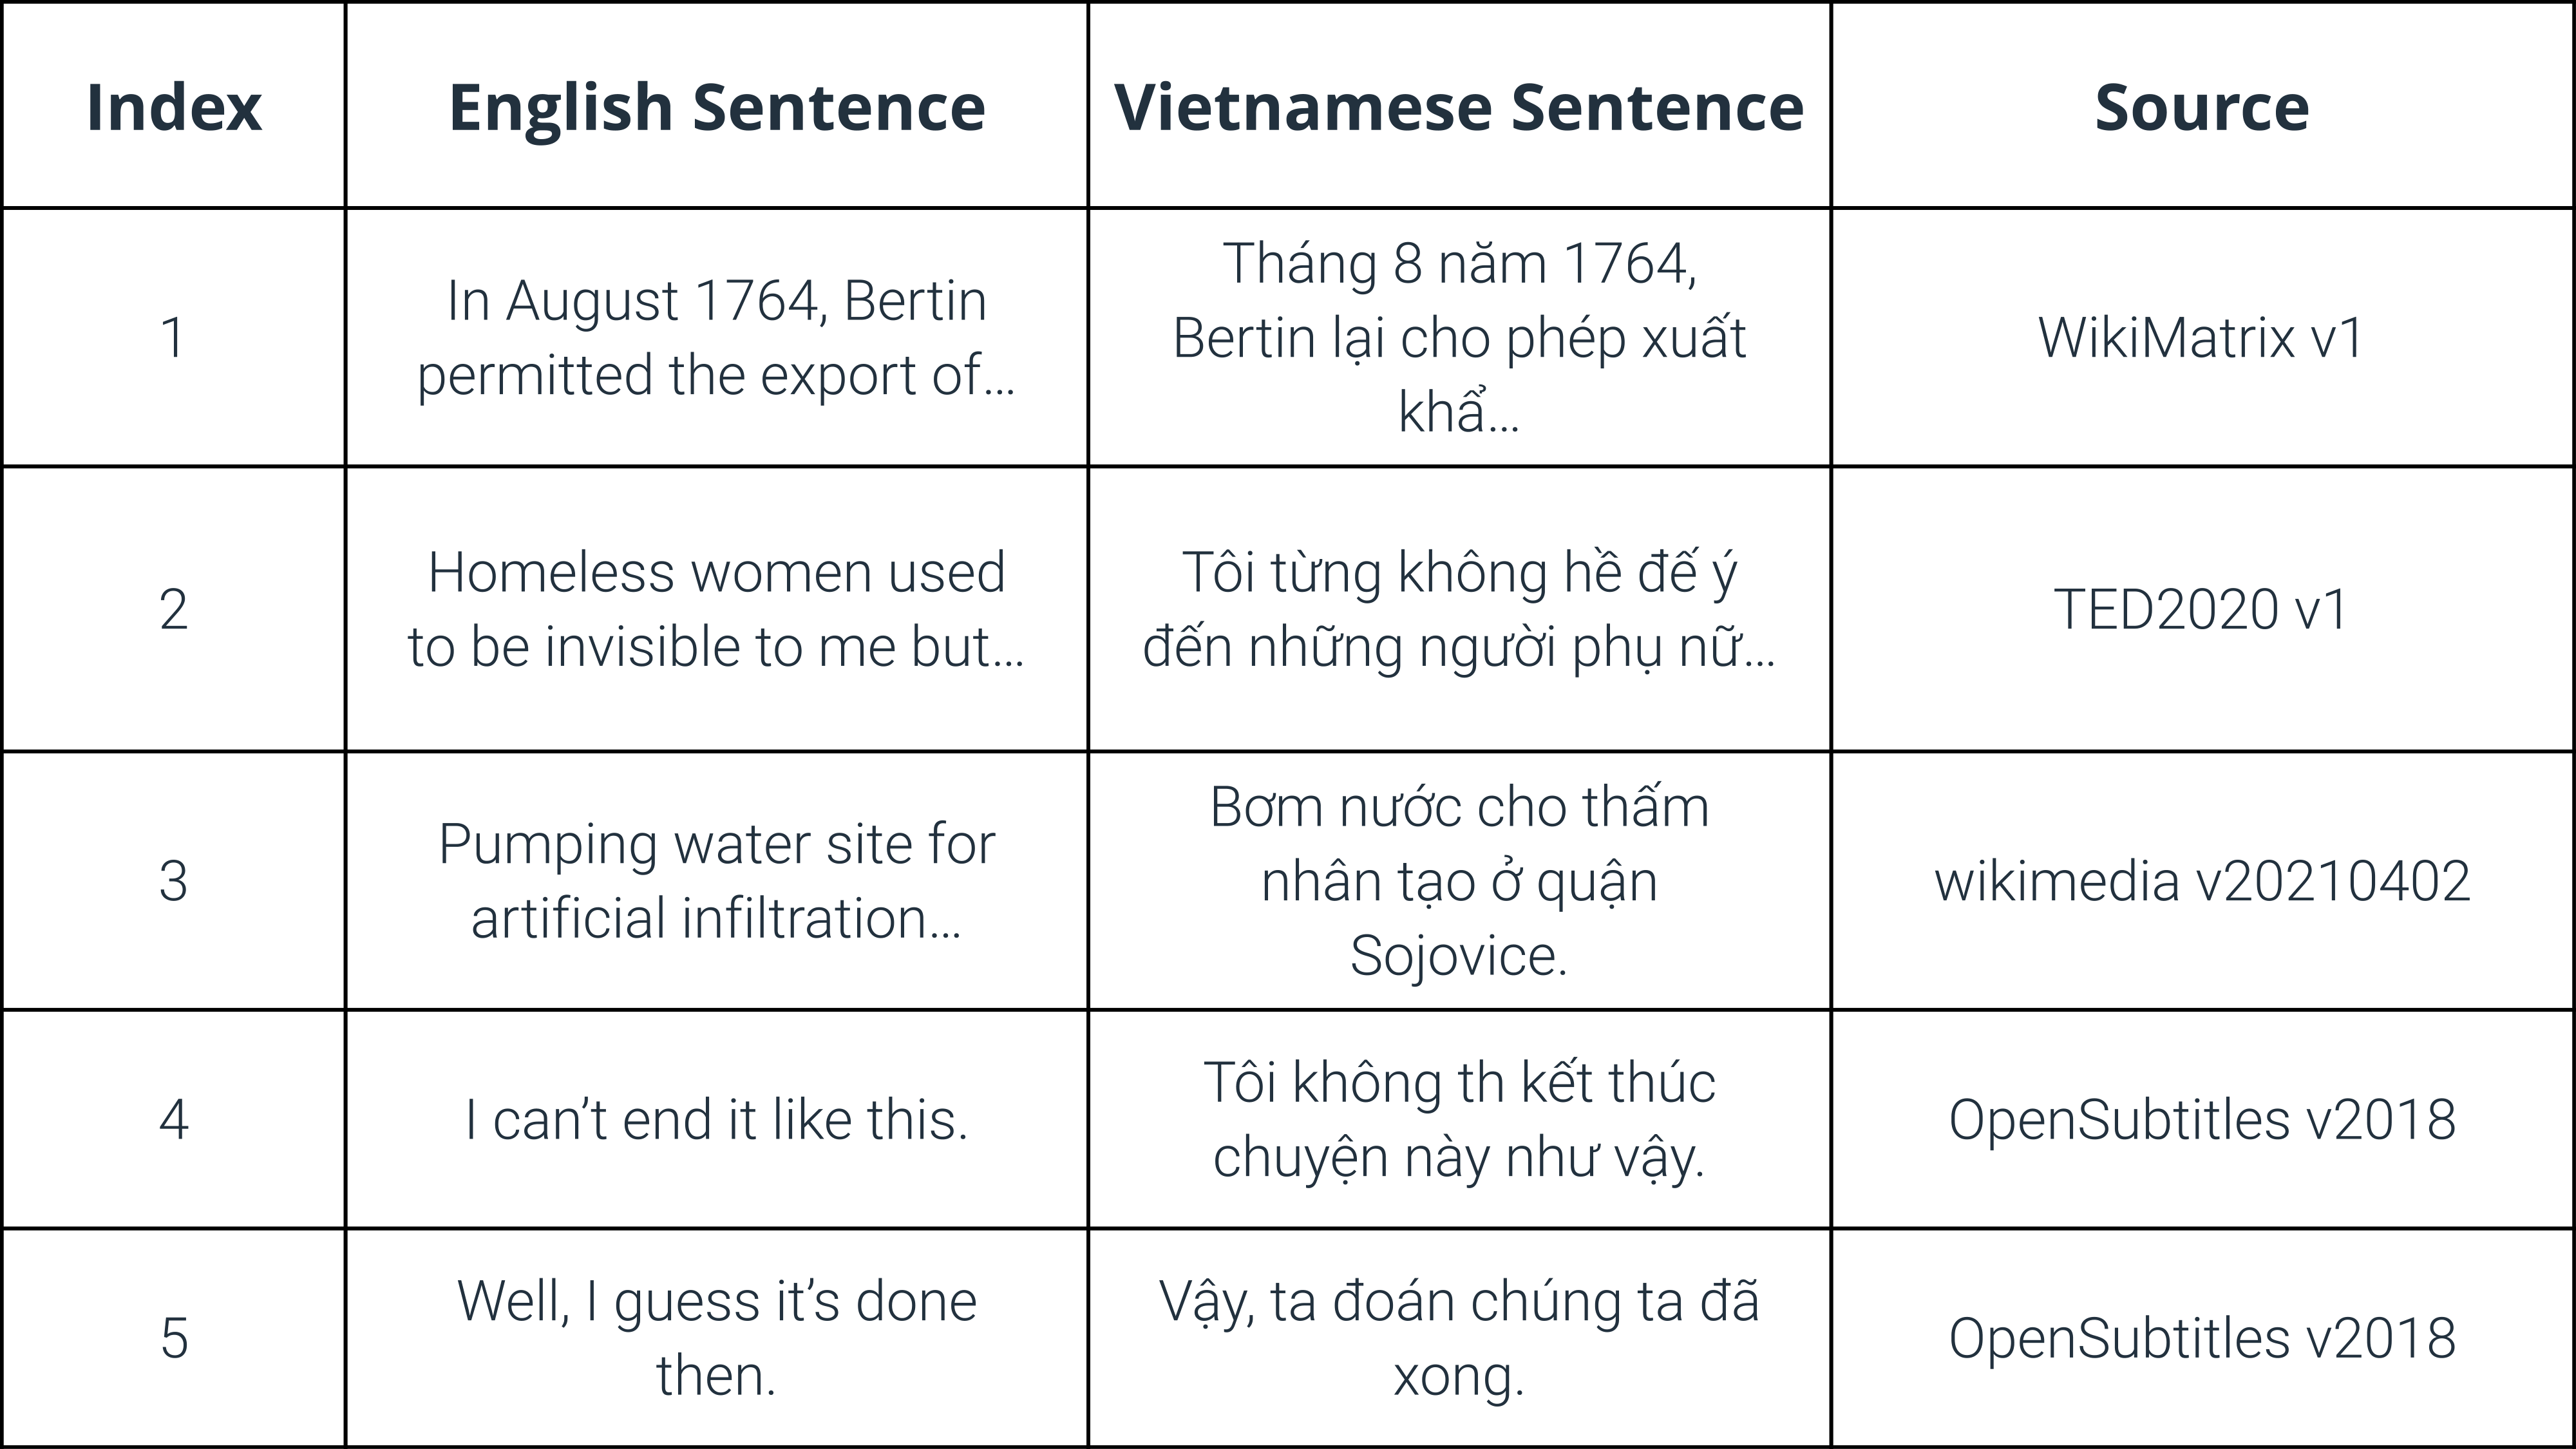
\includegraphics[width=1\linewidth]{figs/head5sample.png} % Thay thế bằng tên file hình ảnh của bạn
    \caption{Head 5 Samples of Training Data}
    \label{fig:training-data}
\end{figure}
The provided image showcases a table from a dataset containing paired English and Vietnamese sentences used for machine translation. The table includes five indexed rows, each with an English sentence, its corresponding Vietnamese translation, and the source from which the sentence pair was obtained. 

\textbf{Dataset Shapes:}
\begin{itemize}
\item Train data shape: (200000, 2)
\item Valid data shape: (11316, 2)
\item Test data shape: (11225, 2)
\end{itemize}

\subsection{Data Analysis}


\begin{figure}[H]
    \centering
    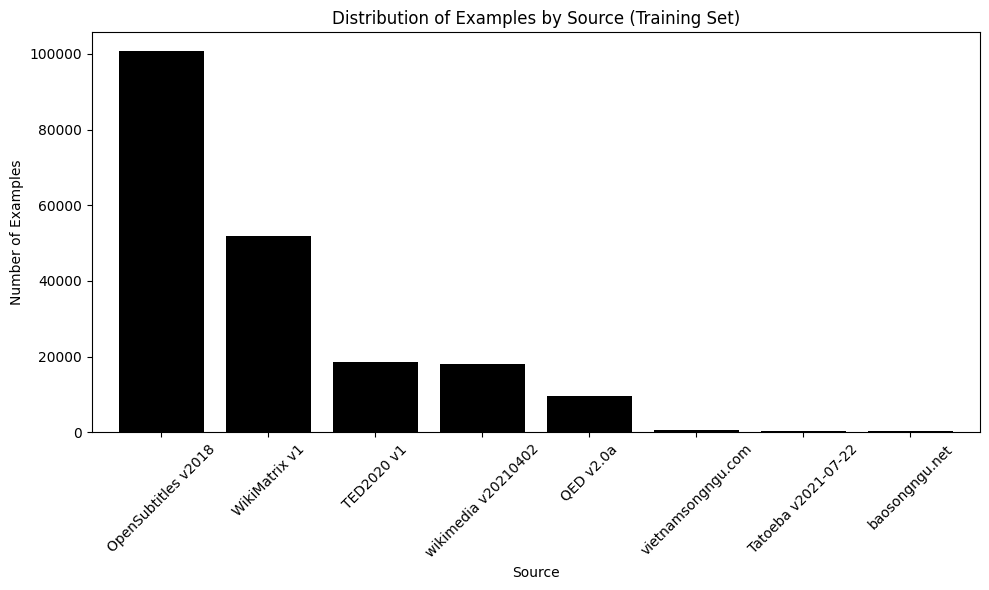
\includegraphics[width=1\textwidth]{figs/source.png} 
    \caption{Distribution of Examples by Source (Training Set)}
\end{figure}
The source "OpenSubtitles v2018" is the most substantial contributor, providing just over 100,000 examples. Following this, "WikiMatrix V1" is the second largest source, offering approximately 50,000 examples. Other significant contributors include "TED2020 V1" and "Wikimedia v20180402," each providing around 10,000 examples. The "QED v2.0a" source offers just under 10,000 examples. Several other sources, namely "vietnamsongngu.com," "Tatoeba v2021-07-22," and "baosongngu.net," contribute a minimal number of examples, barely noticeable on the chart.

\begin{figure}[H]
    \centering
    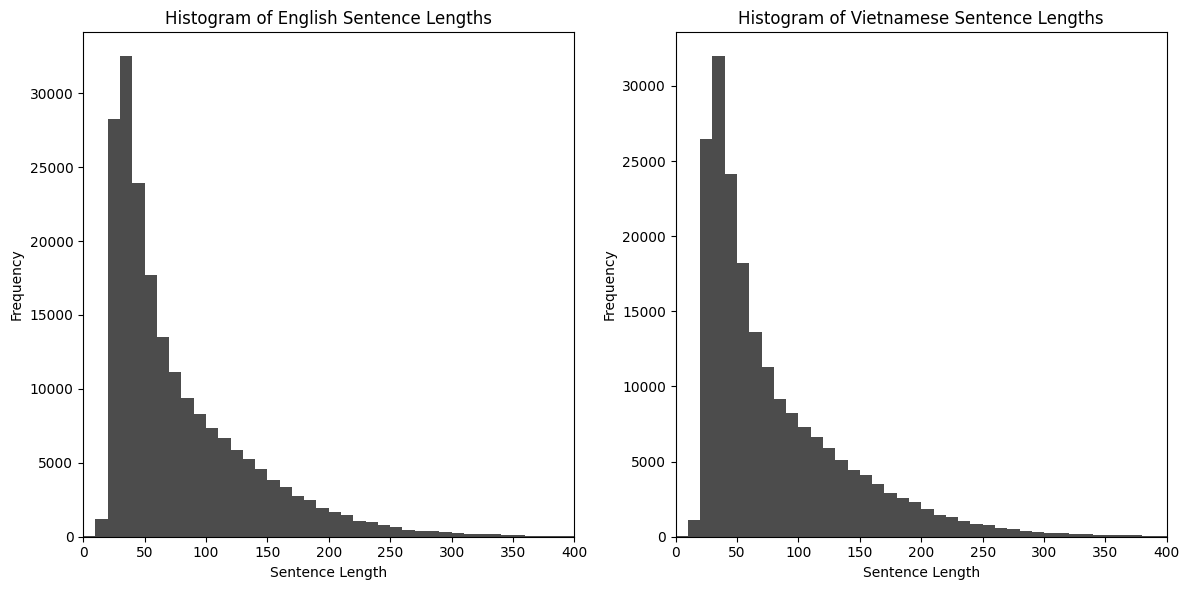
\includegraphics[width=1\textwidth]{figs/histogram.png}
    \caption{Lengths of English and Vietnamese sentences}
\end{figure}
The histogram on the left, titled "Histogram of English Sentence Lengths," displays the frequency of English sentence lengths. The x-axis represents the sentence length, while the y-axis denotes the frequency of each length. The distribution shows a steep decline, with the majority of sentences falling between 0 and 50 characters. The frequency decreases significantly as the sentence length increases, indicating a higher concentration of shorter sentences within the dataset. The highest frequency, approximately 30,000 sentences, occurs at the shorter lengths, with a long tail extending towards longer sentences, which are considerably less frequent.

Similarly, the histogram on the right, titled "Histogram of Vietnamese Sentence Lengths," shows a comparable distribution pattern for Vietnamese sentences. The majority of sentences again fall between 0 and 50 characters, with a frequency peak at around 30,000 sentences. As the sentence length increases, the frequency diminishes, following a similar long-tailed distribution as observed with the English sentences.

Both histograms reveal a common characteristic in natural language corpora where shorter sentences are more prevalent than longer ones. This distribution is crucial for understanding the dataset's structure, aiding in designing and optimizing machine translation models to handle varying sentence lengths effectively. The parallel patterns in English and Vietnamese sentence lengths suggest a consistent methodology in dataset creation, ensuring balanced and comparable data for training purposes.

\begin{figure}[H]
    \centering
    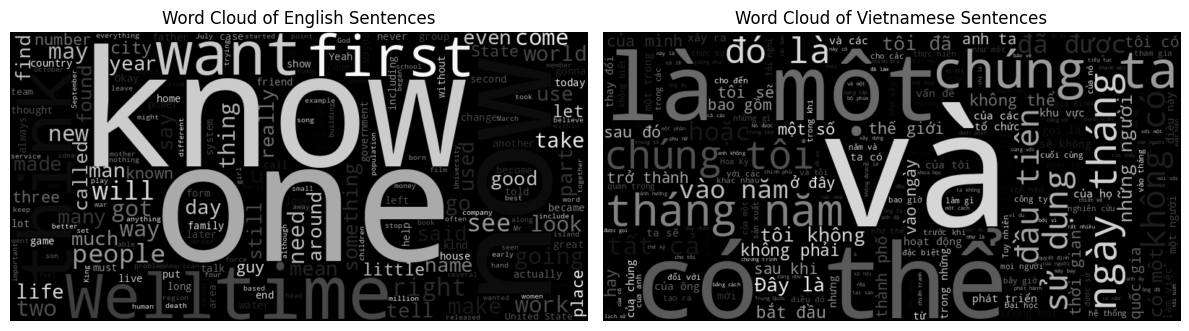
\includegraphics[width=1\textwidth]{figs/wordcloud.png}
    \caption{Word Clouds of English and Vietnamese Sentences}
\end{figure}
The word cloud on the left, labeled "Word Cloud of English Sentences," displays a prominent visualization of common English words. Larger words signify higher frequency within the dataset. Key words such as "know," "one," "first," "want," and "we" appear prominently, indicating their frequent usage. Other notable words include "day," "people," "new," "life," and "year." This distribution highlights common themes and vocabulary in the English sentences, reflecting everyday conversational and contextual usage.

On the right, the 'Word Cloud of Vietnamese Sentences' depicts the prevalent words in Vietnamese. Similar to the English word cloud, larger words represent higher frequency. Words like 'va' (and), 'la' (is/are), 'mot' (one/a), 'co' (have/there is), and 'thang' (month) stand out prominently. Additional frequent words include 'nam' (year), 'toi' (I), 'chung' (we), 'khong' (not), and 'ngay' (day). This visualization reveals the common vocabulary used in Vietnamese sentences, capturing essential elements of everyday language and context

\subsection{Model Settings}
The table below compares key settings for the models.

\begin{table}[H]
\centering
\begin{tabular}{|c|c|c|c|}
\hline
\textbf{Model} & \textbf{Batch Size} & \textbf{Epochs} & \textbf{Learning Rate} \\
\hline
Seq2Seq RNN & 32 & 5 & 0.0005 \\
Transformer & 30 & 5 & 0.00001 \\
MarianMT & 16 & 5 & 0.00005 \\
\hline
\end{tabular}
\caption{Comparison of Model Settings for Machine Translation}
\label{table:model_settings}
\end{table}

\begin{table}[H]
\centering
\begin{tabular}{|c|c|c|}
\hline
\textbf{Model} & \textbf{Loss Function} & \textbf{Optimizer} \\
\hline
Seq2Seq RNN & Cross-Entropy Loss & Adam \\
Transformer & Cross-Entropy Loss & Adam \\
MarianMT & Cross-Entropy Loss & AdamW \\
\hline
\end{tabular}
\caption{Comparison of Loss Functions and Optimizers for Machine Translation}
\label{table:loss_optimizer}
\end{table}
For the Seq2Seq RNN model, we opted for a batch size of 32 to balance between computational efficiency and model convergence during training over 5 epochs. A moderate learning rate of 0.0005 was chosen to facilitate steady learning without compromising stability.

The Transformer model, known for its parallel processing capabilities, utilized a slightly reduced batch size of 30 to efficiently handle the computational demands inherent in its architecture. With a lower learning rate of 0.00001, we aimed to fine-tune the Transformer's extensive parameters over 5 epochs, leveraging its self-attention mechanism to capture complex translation patterns effectively.

For MarianMT, our implementation considered a batch size of 16 to accommodate its efficient memory utilization while training for 5 epochs. A learning rate of 0.00005, coupled with the AdamW optimizer for weight decay regularization, was specifically chosen to optimize performance and mitigate overfitting in our training regimen.

Each model employed a Cross-Entropy Loss function paired with appropriate optimizers—Adam for Seq2Seq RNN and Transformer, and AdamW for MarianMT. These selections were tailored to suit the respective model architectures and training paradigms, ensuring effective gradient descent and parameter updates throughout the training process.

\subsubsection{RNN-based Seq2Seq}
Seq2Seq models use RNNs for both the encoder and decoder to process input and output sequences, respectively. Our Seq2Seq model consists of:

\begin{itemize}
\item \textbf{Embedding Layers:} For both input and output sequences.
\item \textbf{Encoder:} Two-layer bidirectional LSTM with 512 hidden units.
\item \textbf{Decoder:} Two-layer LSTM with 512 hidden units.
\item \textbf{Dropout:} 0.5 for both encoder and decoder.
\end{itemize}

\subsubsection{Training Details}
We train the model on the English-Vietnamese dataset with the following parameters:

\begin{itemize}
\item \textbf{Batch Size:} 32.
\item \textbf{Optimizer:} Adam.
\item \textbf{Loss Function:} Cross-Entropy Loss (ignoring padding index).
\end{itemize}

\subsubsection{Transformer for Translation}
The Transformer model uses self-attention to process input and output sequences efficiently.

\begin{itemize}
\item \textbf{Embedding Layers:} For both input and output tokens.
\item \textbf{Transformer Layers:} 2 encoder and 2 decoder layers.
\item \textbf{Hidden Size:} 512.
\item \textbf{Number of Heads:} 8.
\item \textbf{Dropout:} 0.1.
\end{itemize}

\subsubsection{Training Details}
We train the Transformer model on the English-Vietnamese dataset with the following parameters:

\begin{itemize}
\item \textbf{Batch Size:} 30.
\item \textbf{Optimizer:} Adam.
\item \textbf{Loss Function:} Cross-Entropy Loss.
\end{itemize}

\subsubsection{MarianMT for Translation}
MarianMT is a pre-trained model from Helsinki-NLP used for efficient translation tasks.

\begin{itemize}
\item \textbf{Model Name:} Helsinki-NLP/opus-mt-en-vi.
\item \textbf{Batch Size:} 16.
\item \textbf{Optimizer:} AdamW.
\item \textbf{Learning Rate:} 0.00005.
\end{itemize}

\subsubsection{Fine Tuning MarianMT}
Recognizing that MarianMT achieved a high BLEU score, we further fine-tuned this model with different settings to optimize its performance.

\begin{itemize}
\item \textbf{Setting 1:}
  \begin{itemize}
  \item \textbf{Batch Size:} 16
  \item \textbf{Epochs:} 5
  \item \textbf{Learning Rate:} 5e-5
  \end{itemize}
\item \textbf{Setting 2:}
  \begin{itemize}
  \item \textbf{Batch Size:} 8
  \item \textbf{Epochs:} 5
  \item \textbf{Learning Rate:} 3e-5
  \end{itemize}
\item \textbf{Setting 3:}
  \begin{itemize}
  \item \textbf{Batch Size:} 32
  \item \textbf{Epochs:} 5
  \item \textbf{Learning Rate:} 1e-5
  \end{itemize}
\item \textbf{Setting 4:}
  \begin{itemize}
  \item \textbf{Batch Size:} 8
  \item \textbf{Epochs:} 5
  \item \textbf{Learning Rate:} 3e-5
  \item \textbf{Optimizer:} SGD with momentum 0.9
  \end{itemize}
\item \textbf{Setting 5:}
  \begin{itemize}
  \item \textbf{Batch Size:} 16
  \item \textbf{Epochs:} 5
  \item \textbf{Learning Rate:} 3e-5
  \item \textbf{Optimizer:} Adagrad
  \end{itemize}
\end{itemize}

\subsection{Results}
The tables below summarize the training and validation performance of the Seq2Seq RNN, Transformer, and MarianMT models, including the fine-tuned versions of MarianMT.

\begin{table}[H]
\centering
\begin{tabular}{|c|c|c|c|}
\hline
\textbf{Epoch} & \textbf{Seq2Seq RNN} & \textbf{Transformer} & \textbf{MarianMT (Setting 1)} \\
\hline
1 & 5.146 & 1.231 & 0.6745 \\
2 & 4.521 & 0.963 & 0.4604 \\
3 & 4.230 & 0.836 & 0.3884 \\
4 & 4.035 & 0.751 & 0.3355 \\
5 & 3.894 & 0.691 & 0.2947 \\
\hline
\end{tabular}
\caption{Comparison of Training Loss for Seq2Seq RNN, Transformer, and MarianMT (Setting 1) Models}
\end{table}

\begin{table}[H]
\centering
\begin{tabular}{|c|c|c|c|}
\hline
\textbf{Epoch} & \textbf{Seq2Seq RNN} & \textbf{Transformer} & \textbf{MarianMT (Setting 1)} \\
\hline
1 & 5.083 & 1.018 & 0.4787 \\
2 & 4.806 & 0.855 & 0.4044 \\
3 & 4.646 & 0.763 & 0.3623 \\
4 & 4.582 & 0.710 & 0.3356 \\
5 & 4.521 & 0.678 & 0.3186 \\
\hline
\end{tabular}
\caption{Comparison of Validation Loss for Seq2Seq RNN, Transformer, and MarianMT (Setting 1) Models}
\end{table}
In evaluating the performance of the Seq2Seq RNN, Transformer, and MarianMT models for machine translation, it becomes evident that each model
exhibits distinct characteristics in handling training and validation phases. The
Seq2Seq RNN, a traditional architecture in sequence-to-sequence tasks, shows
steady improvement in training loss over epochs, starting with higher values
around 5.1 and gradually reducing to approximately 3.9 by the fifth epoch.
However, its validation losses, though improving similarly, reflect challenges in
generalizing to unseen data as they start higher and reduce more modestly compared to the Transformer and MarianMT models.
In contrast, the Transformer model, renowned for its self-attention mechanisms and parallel processing capabilities, begins training with significantly
lower loss values, approximately 1.2, and swiftly converges to about 0.7 by the
fifth epoch. This rapid reduction in both training and validation losses underscores the Transformer’s efficacy in capturing intricate dependencies across
sequences, thereby enhancing its ability to generalize well to new data.
Yet, the most striking performance emerges from the MarianMT model,
particularly in its fine-tuned settings. Starting with an initial training loss
as low as 0.67, MarianMT achieves remarkable refinement, culminating in a
training loss of approximately 0.29 by the fifth epoch. Equally impressive, its
validation loss mirrors this trend, starting near 0.48 and steadily decreasing to
about 0.32. This demonstrates MarianMT’s robust adaptation to the translation
task, leveraging its pre-trained knowledge and optimizing it through fine-tuning
for specific nuances in the dataset.

\begin{table}[H]
\centering
\begin{tabular}{|c|c|c|c|c|c|}
\hline
\textbf{Epoch} & \textbf{Setting 1} & \textbf{Setting 2} & \textbf{Setting 3} & \textbf{Setting 4} & \textbf{Setting 5} \\
\hline
1 & 0.6745 & 0.6627 & 1.1661 & 1.2432 & 1.0755 \\
2 & 0.4604 & 0.4622 & 0.7292 & 1.0059 & 0.8720 \\
3 & 0.3884 & 0.3924 & 0.6431 & 0.9450 & 0.8241 \\
4 & 0.3355 & 0.3410 & 0.5909 & 0.9066 & 0.7917 \\
5 & 0.2947 & 0.3007 & 0.5550 & 0.8795 & 0.7680 \\
\hline
\end{tabular}
\caption{Comparison of Training Loss for Different Settings of MarianMT}
\end{table}

\begin{table}[H]
\centering
\begin{tabular}{|c|c|c|c|c|c|}
\hline
\textbf{Epoch} & \textbf{Setting 1} & \textbf{Setting 2} & \textbf{Setting 3} & \textbf{Setting 4} & \textbf{Setting 5} \\
\hline
1 & 0.4787 & 0.4798 & 0.7566 & 1.0118 & 0.8618 \\
2 & 0.4044 & 0.4073 & 0.6424 & 0.9294 & 0.8011 \\
3 & 0.3623 & 0.3662 & 0.5812 & 0.8833 & 0.7641 \\
4 & 0.3356 & 0.3394 & 0.5412 & 0.8529 & 0.7377 \\
5 & 0.3186 & 0.3222 & 0.5142 & 0.8303 & 0.7176 \\
\hline
\end{tabular}
\caption{Comparison of Validation Loss for Different Settings of MarianMT}
\end{table}
In the initial epochs, the training losses for the different settings display noticeable variation. Setting 1, which employs a batch size of 16 and a learning rate of 5e-5, starts with a moderate training loss of 0.6745. In contrast, Setting 3, with a batch size of 32 and a lower learning rate of 1e-5, exhibits a significantly higher initial training loss of 1.1661, indicating slower convergence. Similarly, Setting 4, which utilizes SGD with momentum, begins with the highest training loss of 1.2432. This suggests that larger batch sizes or different optimizers may require more epochs to reach optimal performance.

As training progresses, the trends in loss reduction become clearer. Setting 1 consistently demonstrates efficient loss reduction, achieving the lowest final training loss of 0.2947 by epoch 5. This highlights the effectiveness of a balanced batch size and a relatively higher learning rate in facilitating faster convergence. Conversely, Setting 3 continues to lag, ending with a higher training loss of 0.5550, underscoring the challenges posed by its larger batch size and lower learning rate combination.

The validation losses across different settings follow a similar pattern to the training losses. Setting 1 again performs well, starting with a validation loss of 0.4787 and decreasing steadily to 0.3186 by epoch 5. Setting 4, despite its initial high training loss, shows a significant reduction in validation loss over epochs, reaching 0.8303, which is notably higher than the other settings. This indicates that while SGD with momentum may initially hinder rapid convergence, it can still achieve reasonable validation performance with sufficient training.

\begin{table}[H]
\centering
\begin{tabular}{|c|c|}
\hline
\textbf{Model} & \textbf{Test BLEU Score} \\
\hline
Seq2Seq RNN & 4.7 \\
Transformer & 13.49 \\
MarianMT (Setting 1) & 47.49 \\
MarianMT (Setting 2) & 34.78 \\
MarianMT (Setting 3) & 8.25 \\
MarianMT (Setting 4) & 74.45 \\
MarianMT (Setting 5) & 64.48 \\
\hline
\end{tabular}
\caption{Comparison of Test BLEU Scores for Different Models and Settings}
\label{table:test_bleu_scores}
\end{table}


In assessing the test BLEU scores across various models, a distinct hierarchy emerges, elucidating their varying capabilities in machine translation tasks. The Seq2Seq RNN model achieves a modest BLEU score of 4.7, indicating its limited proficiency in accurate text translation compared to more sophisticated architectures. In contrast, the Transformer model significantly enhances translation quality with a BLEU score of 13.49, underscoring the efficacy of its self-attention mechanism in capturing contextual dependencies and improving translation accuracy. However, the MarianMT model stands out prominently, demonstrating remarkable BLEU scores across different configurations.

Further analysis of the test BLEU scores highlights the significant impact of different settings. Setting 4, despite initially higher losses, achieves the highest test BLEU score of 74.45, suggesting that the use of SGD optimizer with momentum notably enhances translation quality. Conversely, Setting 1, while effective in reducing losses, yields a test BLEU score of 47.49, indicating that its configuration, although conducive to convergence, may not optimize translation accuracy to the fullest extent.

In conclusion, the fine-tuning of the MarianMT model underscores the effectiveness of exploring diverse configuration strategies. While conventional settings with balanced batch sizes and learning rates facilitate efficient convergence, alternative configurations such as SGD with momentum demonstrate superior translation quality, as evidenced by higher BLEU scores. This highlights the importance of comprehensive exploration in optimizing model performance.
\begin{figure}[H]
    \centering
    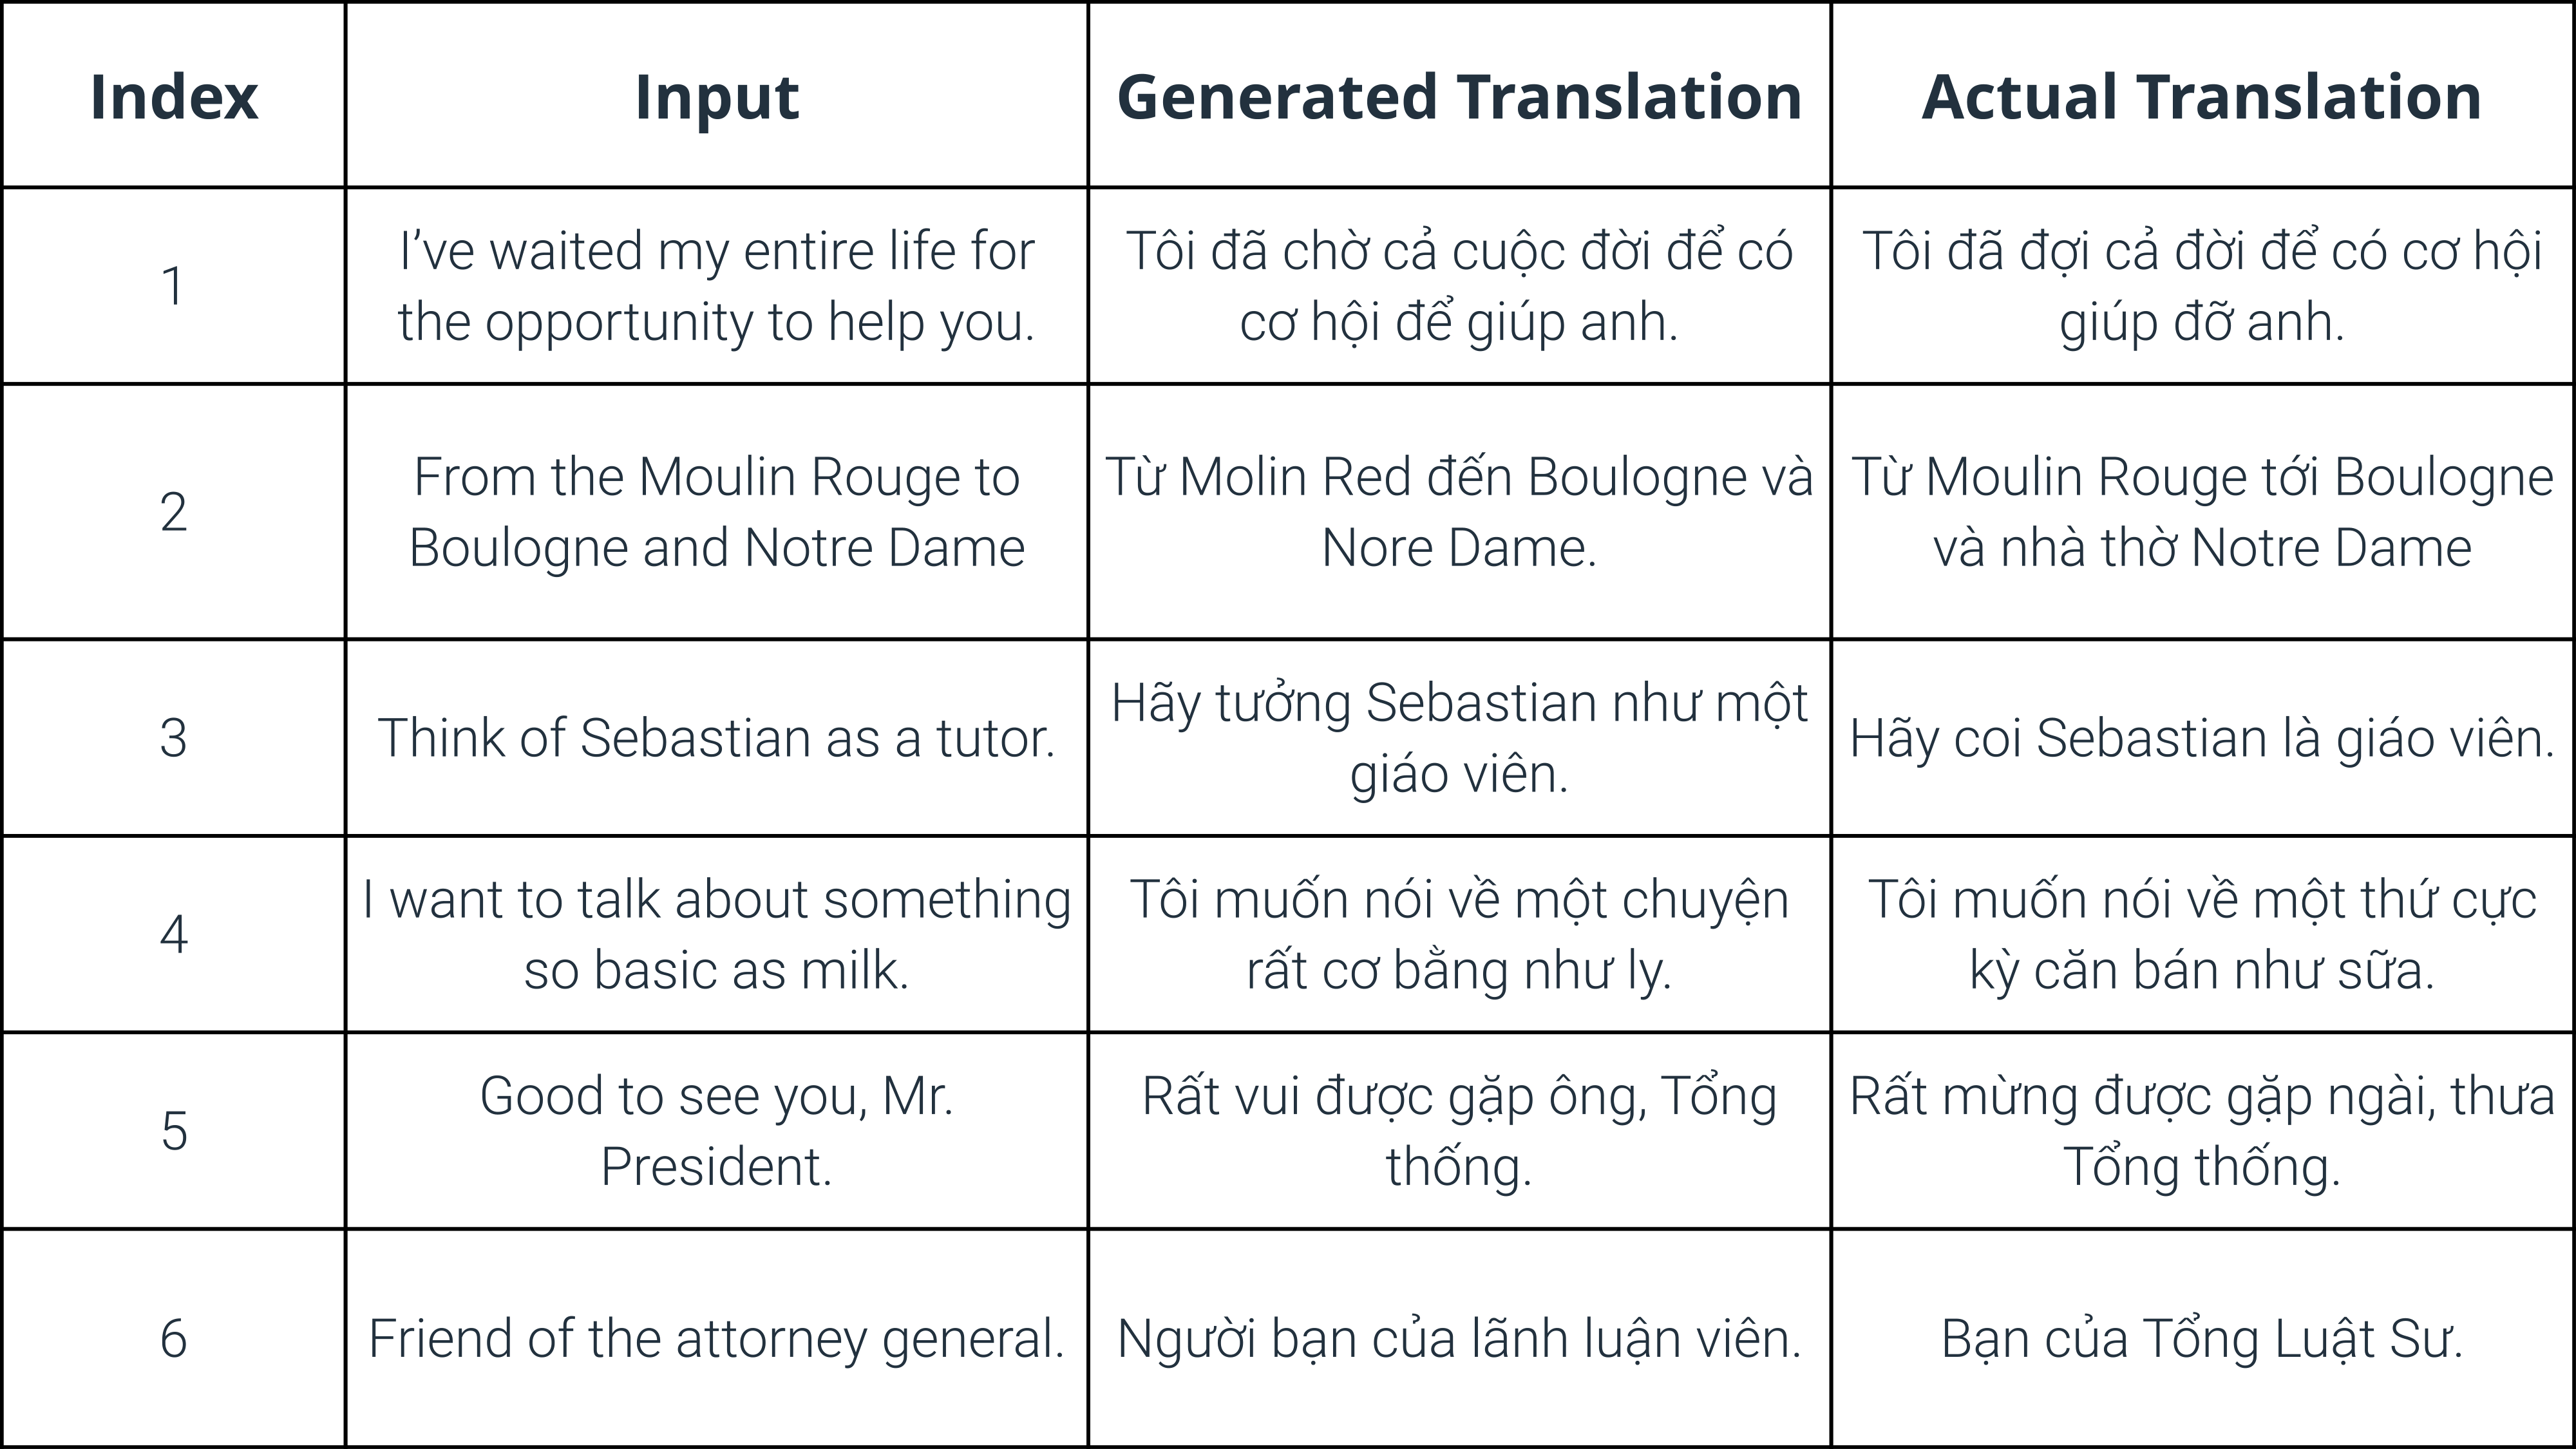
\includegraphics[width=\textwidth]{figs/MarianMT.png}
    \caption{Generated translations from the best fine-tuned MarianMT model compared to the actual translations.}
    \label{fig:MarianMT_comparison}
\end{figure}

The MarianMT model underwent fine-tuning using a batch size of 8 and a learning rate of  $3 \times 10^{-5}$ over 5 epochs, employing the SGD optimizer with a momentum of 0.9. As illustrated  in Figure~\ref{fig:MarianMT_comparison}, the generated translations demonstrate the model's ability to produce coherent and contextually accurate translations. 

In summary, the fine-tuned MarianMT model exhibits strong translation performance, as evidenced by the BLEU scores and the qualitative assessment of the generated translations. The table and figure provide a clear illustration of the improvements achieved through fine-tuning, highlighting the model's potential for practical machine translation applications.

\section{Analysis and Discussion}
\subsection{Sentiment Analysis}
The inclusion of diverse neural network architectures such as RNNs, LSTM, GRU, Bidirectional LSTM, Transformer, and Fine-Tuned Transformer marks a significant advancement in our NLP project. Each architecture brings unique strengths to sentiment analysis tasks, as evidenced by their respective performance metrics. RNNs, while foundational, exhibit limitations in capturing long-term dependencies and intricate language nuances. For instance, the RNN model achieved a test accuracy of 82.82\%, suggesting moderate performance in sentiment classification tasks. LSTMs and GRUs, with their enhanced ability to retain information over longer sequences, outperform traditional RNNs. The LSTM model achieved a commendable test accuracy of 85.84\%, highlighting its efficacy in capturing and utilizing contextually rich information. The Bidirectional LSTM, by processing sequences in both forward and backward directions, further improves upon LSTM's performance. It achieved a notable test accuracy of 86.96\%, indicating its robustness in understanding contextual dependencies across sentences. Transformers represent a paradigm shift in NLP, leveraging self-attention mechanisms to capture global dependencies efficiently. Our custom Transformer architecture achieved a competitive test accuracy of 85.55\%, demonstrating its capability to handle diverse language patterns effectively. The Fine-Tuned Transformer, leveraging pre-trained models and specialized fine-tuning, emerged as the top performer in our analysis. With an impressive test accuracy of 92.80\%, it significantly surpasses other models, underscoring the power of transfer learning in NLP tasks.

\subsection{Machine Translation}
In the realm of machine translation, our findings reveal a striking performance gap between traditional Seq2Seq RNN models and more modern approaches. The Transformer model, with its parallel processing capabilities and self-attention mechanism, achieved a BLEU score of 13.49, indicating a substantial improvement over the Seq2Seq RNN model, which only reached a BLEU score of 4.7. However, it was the fine-tuned MarianMT model that truly excelled. Among the fine-tuned settings, MarianMT Setting 4, employing a batch size of 8, a learning rate of 3e-5, and optimized with SGD with momentum 0.9, achieved the highest BLEU score of 74.45. This demonstrates the model's capacity to generate coherent, contextually accurate translations, surpassing the BLEU scores of both the Seq2Seq RNN and the Transformer models. These results underscore the effectiveness of leveraging large-scale pre-trained models and fine-tuning them for specific tasks to achieve state-of-the-art results.

\section{Conclusion}
In conclusion, this study has explored a variety of advanced neural network architectures for both sentiment analysis and machine translation tasks. Through the evaluation of models such as RNNs, LSTMs, GRUs, Bidirectional LSTMs, Transformers, and Fine-Tuned Transformers, we have observed their distinct capabilities in handling sequential data and capturing intricate dependencies across texts.

For sentiment analysis, these architectures have demonstrated varying levels of effectiveness in understanding and classifying sentiment. Traditional models like RNNs provide a foundational understanding but are surpassed by LSTM and GRU models, which excel in retaining contextual information over longer sequences. The Bidirectional LSTM further enhances performance by processing information in both forward and backward directions, thus capturing richer contextual dependencies. The introduction of Transformers marks a significant advancement, leveraging self-attention mechanisms to efficiently capture global dependencies and achieve competitive performance. Notably, the Fine-Tuned Transformer model emerges as the top performer, leveraging transfer learning to achieve superior accuracy.

In the realm of machine translation, our study contrasts traditional Seq2Seq RNNs with more modern approaches such as Transformers and the fine-tuned MarianMT model. While Transformers demonstrate substantial improvements in translation accuracy over Seq2Seq RNNs, the MarianMT model, particularly in its fine-tuned configurations, surpasses both, highlighting the efficacy of large-scale pre-trained models and fine-tuning for achieving contextually accurate translations.

Overall, this research underscores the transformative impact of advanced neural network architectures in natural language processing tasks. The findings emphasize the importance of model selection based on task requirements and the potential of transfer learning and fine-tuning in optimizing model performance. Future studies may explore hybrid approaches and ensemble methods to further enhance the versatility and robustness of NLP applications across various domains and languages.
\section{References}
\begin{thebibliography}{9}
\bibitem{vaswani2017attention} Vaswani, Ashish, et al. "Attention is all you need." Advances in neural information processing systems 30 (2017).
\bibitem{devlin2018bert} Devlin, Jacob, et al. "BERT: Pre-training of Deep Bidirectional Transformers for Language Understanding." arXiv preprint arXiv:1810.04805 (2018).
\bibitem{hochreiter1997long} Hochreiter, Sepp, and Jürgen Schmidhuber. "Long short-term memory." Neural computation 9.8 (1997): 1735-1780.
\bibitem{maas2011learning} Maas, Andrew L., et al. "Learning word vectors for sentiment analysis." Proceedings of the 49th annual meeting of the association for computational linguistics: Human language technologies (2011).
\end{thebibliography}

\end{document}
